\subsection*{Question 3.7}
We are to estimate the density of the second principal component. From
the figure \ref{fig:q37histograms} we see various histograms with
different numbers of bins. Our best guess is around $12$ or $15$ bins
seems optimal, this depicts a mixture model with two modes. If we have
too small a number of bins we loose the ability to capture the real
underlying distribution, on the other hand if we choose to large a
number of bins we end up with a very spiky histogram that are too
noisy to see the real distribution. So one has to choose some
intermediate number of bins.

\begin{figure}[!htbp]
  \centering
  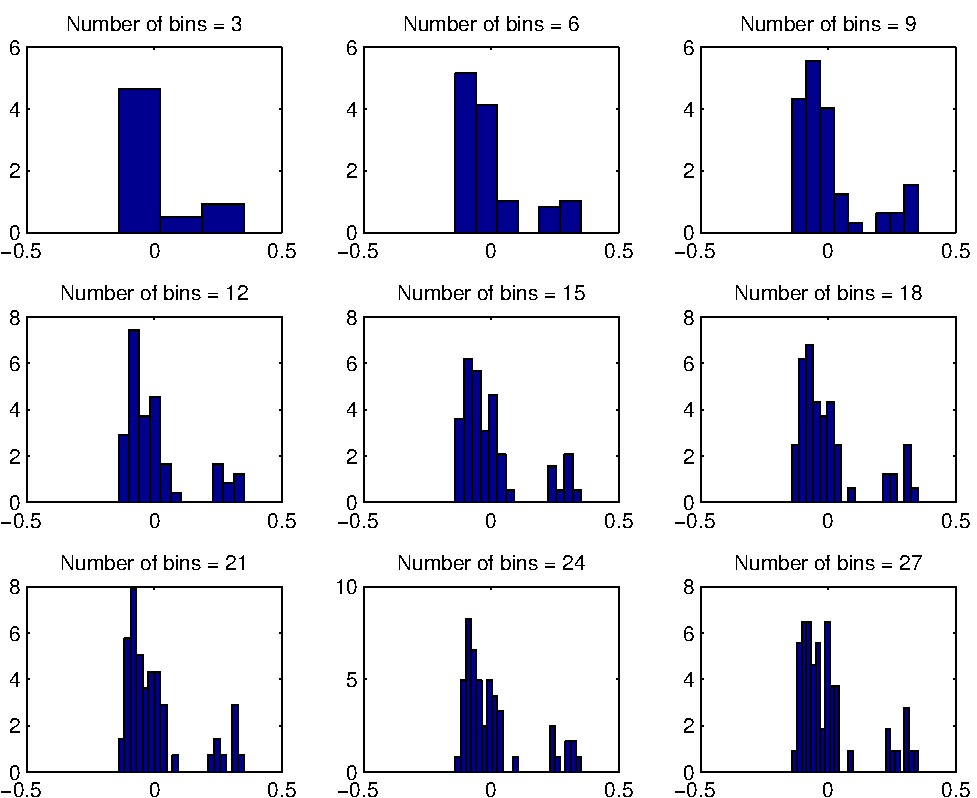
\includegraphics[width=0.85\textwidth]{./images/q37histograms}
  \caption{Shows various histograms.}
  \label{fig:q37histograms}
\end{figure}

Next we are to try out kernel density estimator (kde), this can be
seen in figure \ref{fig:q37kde}. Again we see the same pattern as for
the histogram above. If we choose the bandwidth to be too low this
results in a very spiky structure where and choosing the bandwidth to
large we end up in the same situations as choosing a too small number
of bins. We loose the ability to capture the true form of the
underlying distribution. Some where between $0.03$ and $0.04$ seem to
be the optimal setting for capturing the two modes given by the second
principal component. Using automatic selection the code gives the
optimal bandwidth $0.0329$ which is very close to our best guess, this
can be seen in figure \ref{fig:q37kdeauto}. It is easy to see that
when setting the bandwidth to $>0.05$ the two modes within the data
starts to become one.

\begin{figure}[!htbp]
  \centering
  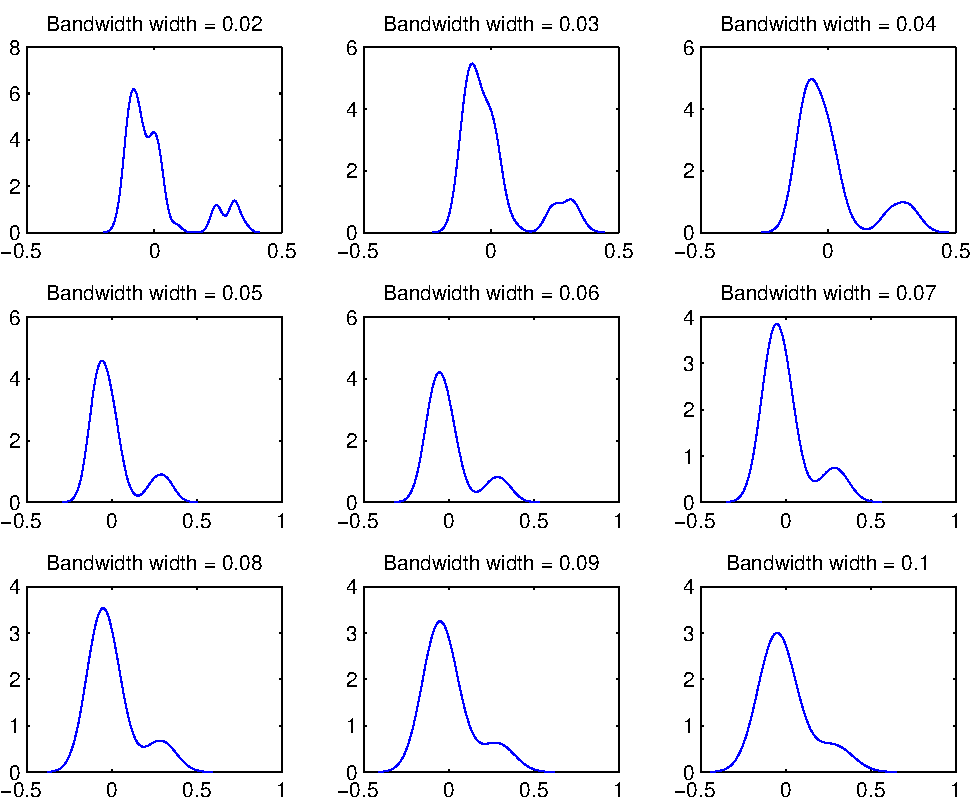
\includegraphics[width=0.85\textwidth]{./images/q37kde}
  \caption{Shows kernel density estimation for various selections of bandwidth.}
  \label{fig:q37kde}
\end{figure}

\begin{figure}[!htbp]
  \centering
  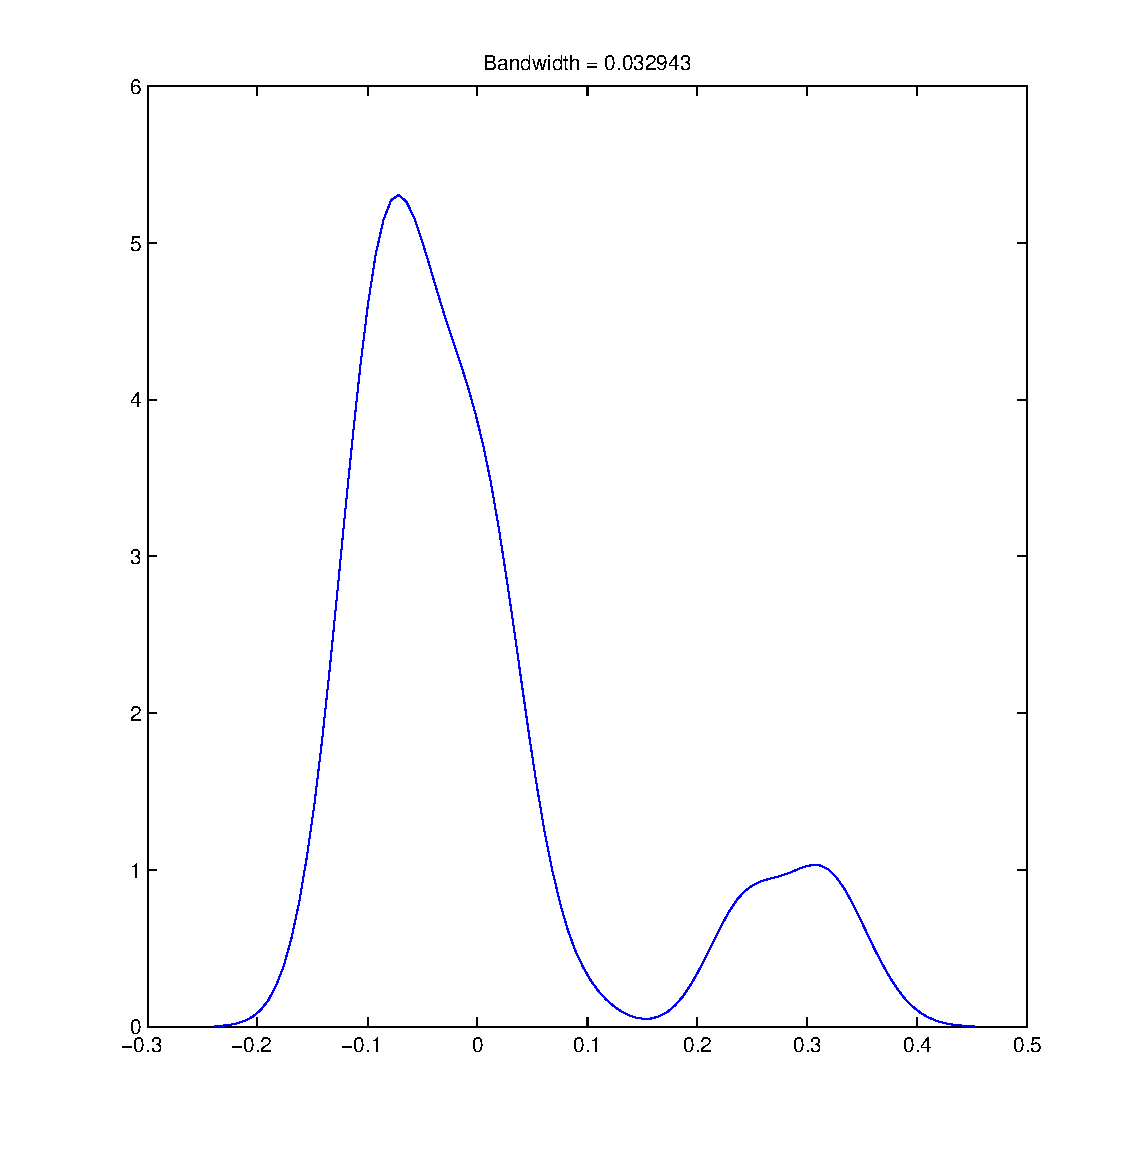
\includegraphics[width=0.6\textwidth]{./images/q37kdeauto}
  \caption{Shows kernel density estimation with automatic bandwidth selection.}
  \label{fig:q37kdeauto}
\end{figure}



\begin{figure}[!htbp]
  \centering
  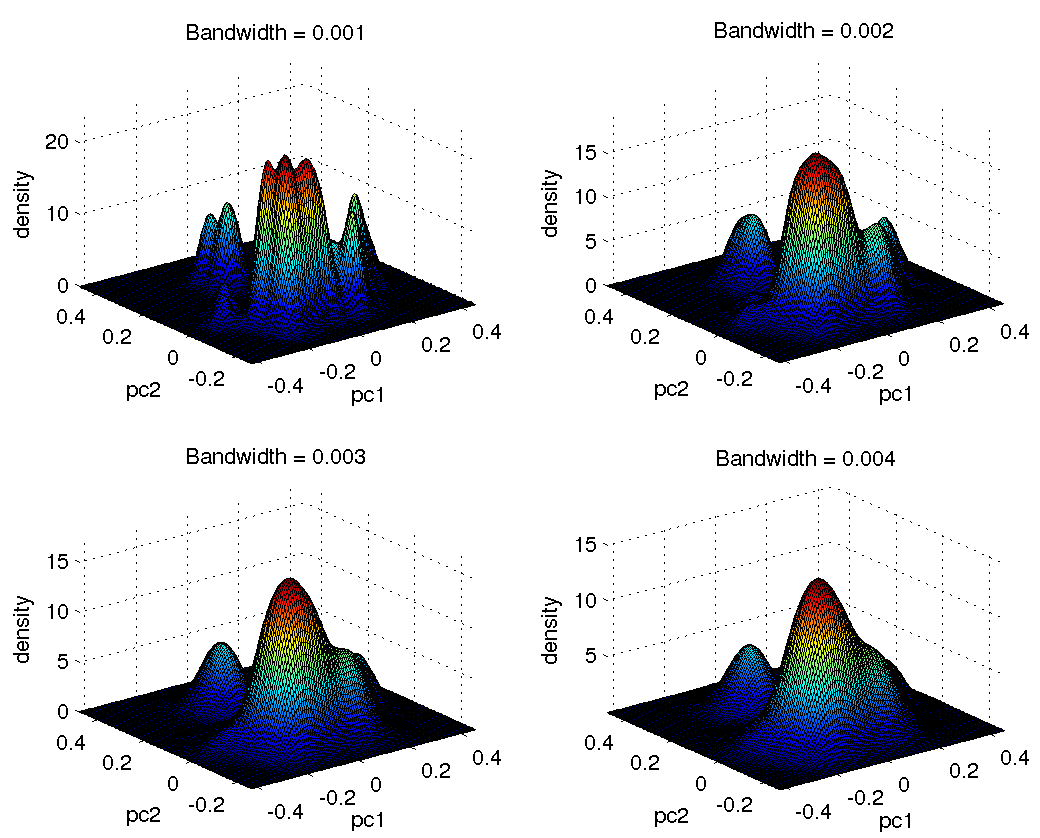
\includegraphics[width=0.6\textwidth]{./images/q373dkde1}
  \caption{Shows 2d kernel density estimations for various selections of bandwidth.}
  \label{fig:q373dkde1}
\end{figure}


\begin{figure}[!htbp]
  \centering
  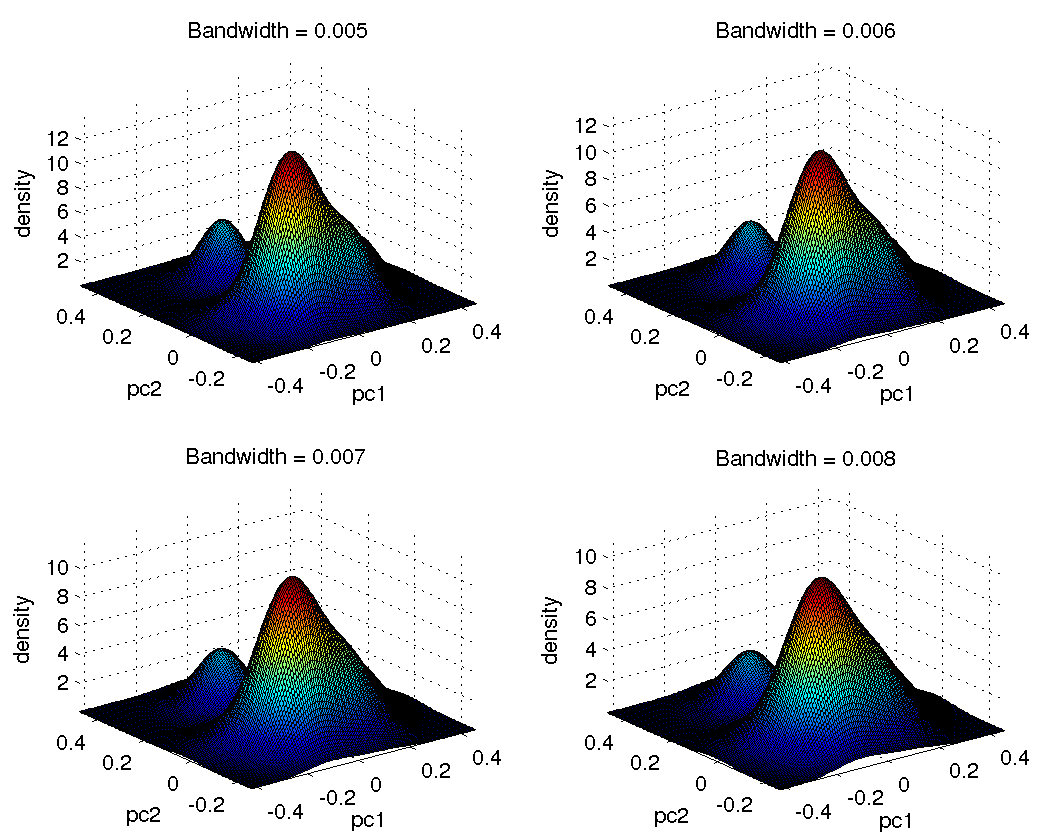
\includegraphics[width=0.6\textwidth]{./images/q373dkde2}
  \caption{Shows 2d kernel density estimations for various selections of bandwidth.}
  \label{fig:q373dkde2}
\end{figure}

